\documentclass[a4paper, 12pt]{article}

%=== Packages ===%

% German language encoding
% \usepackage[ngerman]{babel}
% \usepackage[utf8]{inputenc}
% \usepackage[T1]{fontenc}

% chess board
\usepackage{xskak}

% add graphics
\usepackage{graphicx}

% graphics next to each other
\usepackage{subcaption}

% used for custom enumarations
\usepackage{enumerate}
\usepackage[shortlabels]{enumitem}

% improved tabular package
\usepackage{tabularx}

% for hyperlinks
\usepackage{hyperref}

% Bibliography/Citations
\usepackage{cite}
\usepackage{natbib}

% Draw Pictures
\usepackage{tikz}

\usepackage{ifthen}

%=== Document Setup ===%

% set margin
% use 2cm at the top if no header is used
% use 2.5cm at the bottom if fotter is used
\usepackage[left=3cm, right=2cm, top=2.5cm, bottom=2cm]{geometry}

% headline
\usepackage{fancyhdr}
\usepackage{enumitem}
\usepackage{amsmath}
\usepackage{amssymb}

\pagestyle{fancy}
\fancyhf{}
\rhead{Page \thepage}
\lhead{Creating chess commentary using machine learning}
% \cfoot{}

% for inline code blocks
\usepackage{listings}
\usepackage{xcolor}

\definecolor{backcolour}{RGB}{245, 245, 245}

\lstdefinestyle{codestyle}{
	backgroundcolor=\color{backcolour},
    commentstyle=\color{gray},
    numberstyle=\ttfamily\scriptsize,
    basicstyle=\ttfamily\footnotesize,
    breakatwhitespace=false,         
    breaklines=true,                 
    captionpos=b,                    
    keepspaces=true,                 
    numbers=left,                    
    numbersep=5pt,                  
    showspaces=false,                
    showstringspaces=false,
    showtabs=false,                  
    tabsize=2,
    % xleftmargin=0.15in
}

\lstset{style=codestyle}

\begin{document}

\newgeometry{left=2.5cm, right=2.5cm, top=2.5cm, bottom=2.5cm}

\begin{titlepage}
% University Informations
\begin{flushleft}
Frankfurt University of Applied Sciences\\
Fachbereich 2: Informatik und Ingenieurwissenschaften\\
Informatik (B.Sc.)\\
\end{flushleft}

\vspace{3.5cm}

% Thesis Title
\begin{center}
\Large
\textbf{Creating virtual chess commentators using neural networks}\\
%\large
Subtitle
\end{center}

% Abstract
\begin{abstract}
Computer generated move analysis has become an essential part of today's chess world. This scientific work deals with the question of how neural networks can be used to analyze chess games and create a virtual chess commentator. In particular, we will look at what is needed to represent a chess board that can be used by the neural network to plan and compare moves in order to make an appropriate evaluation of a game of chess. Based on this, we will then explore how the neural network can convert the evaluation into natural language that humans can understand.
\end{abstract}

\vspace{6cm}
	
% Lecturer Informations
\begin{flushright}
Lecturer: Konstantin Ernst\\
Course: Künstliche Intelligenz und wissenschaftliches Arbeiten\\
Winter Semester 22/23\\
\end{flushright}

\vspace{2cm}

% Your Informations
\begin{flushleft}
Submitted by:\\
Max Semdner\\
Matrikelnr.: 1294899\\
\href{mailto: max.semdner@stud.fra-uas.de}{max.semdner@stud.fra-uas.de}\\
\end{flushleft}

\end{titlepage}

\begin{center}
\large
\textbf{Declaration of authorship
}\end{center}

\noindent I hereby certify that the following project report was written entirely by me and is based on my work unless otherwise indicated. I am aware of the University's regulations regarding plagiarism, including the following actions in the event of a violation. Any form of use of outside work is identified where appropriate and noted in the sources.

\vspace{1cm}

\begin{center}
\large
Max Semdner
\end{center}

\begin{tabular}{p{5cm}p{10cm}}
& \\
Approved: & \hrulefill \\
& \\
Date: & \hrulefill \\
\end{tabular}

\restoregeometry

\tableofcontents

\newpage

\section{Introduction}

In the mid-20th century, computer chess experienced its first breakthroughs thanks to the work of scientists like Alan Turing, Claude Shannon and John von Neumann. Alan Turing, the pioneer of artificial intelligence, was convinced that games were an ideal model system for machine learning.\footnote{Cf. \cite{levy-newborn-1982}, pp. 44-45} This prediction has come true, and machine learning have proven to be an essential part of many chess engines today. In particular, recent projects such as AlphaZero, developed by DeepMind, show how efficient programs which use neural networks are in analyzing board games compared to traditionally used algorithms such as alpha-beta search.\footnote{See \cite{alphazero-2018}, p. 1} Although chess engines have become a powerful tool, they have a lack of transparency regarding the moves they perform. Therefore, professional chess players and commentators are often needed to explain the intention of these moves. This dependence on human chess commentators can be a disadvantage, since moves found by computers can sometimes be misinterpreted or not understood at all. Especially for non-professional chess players, many moves played by humans as well as computers are incomprehensible, since they do not have the appropriate experience. In the following, the construction of a chess engine is discussed, which corresponds in its play and analysis strength to the engines of today. This should serve to analyze moves in their depth. Then the construction of a virtual chess commentator is described, which uses the information gained by the analysis of the chess engine to create detailed comments on a given position and move.

\section{Chess Commentator powered by a Neural Network}

\subsection{General Approach}

% In the implementation, it plays an important role what kind and how much information the neural network receives about the analysis of the individual moves in order to generate the most accurate translations possible. This is influenced by the placement of the chess engine, which can be placed either internally or externally. Internal means that the engine works as part of the neural network, which also includes the chess commentator. When placed externally, the neural net is only used for the translations of the chess commentator and uses the analysis of an outside placed engine. In the following, we will only focus on the internal placement, as this achieved the best results. For this reason I, follow the similar model, as described by ...

As described in the next section, each chess engine must meet certain requirements. Based on the requirements, context is generated. Context is a set of properties that apply to the current position on the chess board. These properties are used by the generation models to make comprehensive statements about the moves.

% Wie im nächsten Abschnitt beschrieben, muss jede Schachengine bestimmte Anforderungen erfüllen. Basierend auf den Anforderungen wird Kontext generiert. Bei Kontext handelt es sich um Eigenschaften welche auf die Aktuelle Position auf dem Schachbrett zutreffen. Diese Eigenschaften werden von den Generierungsmodellen verwendet, um umfassende Aussagen über die Züge zu machen.

\subsection{Chess Engine}

Any chess engine must meet a number of requirements in order to function. These requirements include the \textit{representation of the chessboard}, the \textit{prediction of the possible moves} and the \textit{evaluation of the possible moves}. These requirements can be implemented in a number of ways. Certain implementation options have become widely accepted. In the following, one implementation procedure is presented for each requirement. These are state of the art implementations that have been in use for many years or have achieved great success in the recent past. 

\subsubsection{Board Representation}

Since the computer cannot work with a physical chess board and pieces, these must be converted into a form in which the board, pieces, and position can be interpreted by the computer and later used for the input layer of the neural network. The most common way of representing positions and movements of chess pieces is the data structure bitboards. A bitboard is implemented as an $8 \times 8$ bit array, which is the size of a chessboard.\footnote{Cf. \cite{boskovic-2005-bb}, p. 360} Each array element corresponds to a square on the board. A bitboard is created for each type of piece (pawn, knight, bishop, rook, queen and king) of a given color (black and white). Further 4 board for "2 casteling choices of each player"\footnote{\cite{zang-etal-2019-automated}} are generated. This gives a total number of 16 bitboards. Finally, the squares on which the figures are placed must be marked on the respective boards. This can be done in binary, where 0 means the square is empty and 1 means the square is not empty.

\begin{figure}[h]
\centering
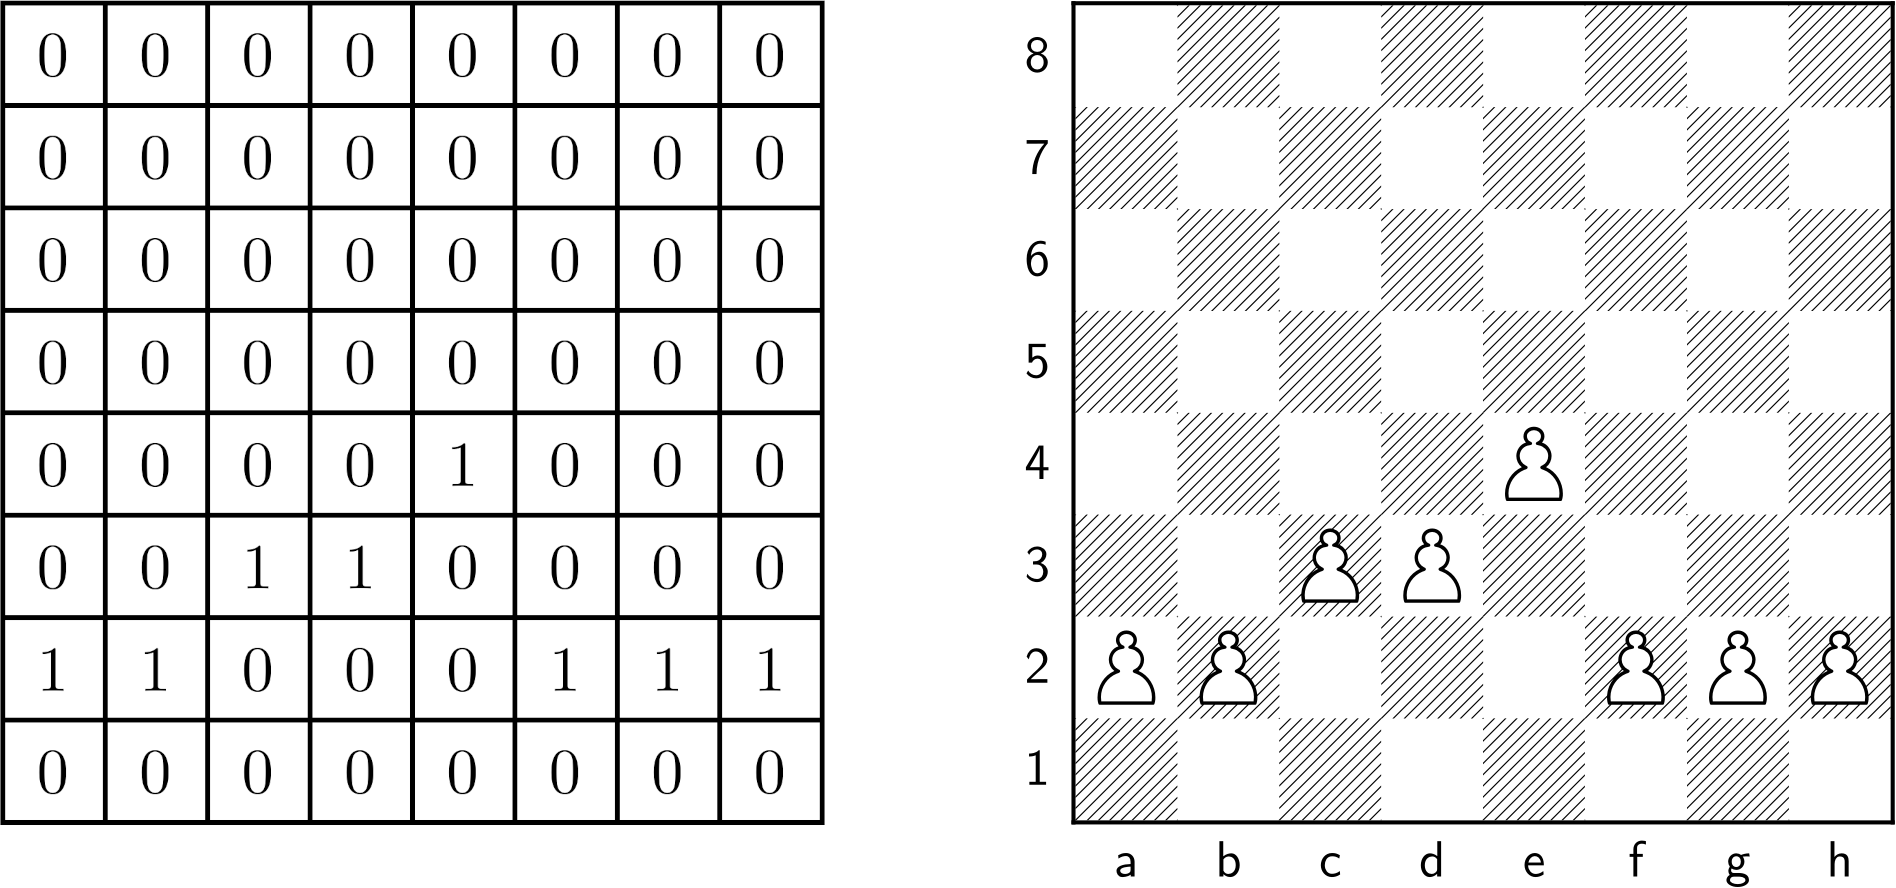
\includegraphics[width=0.5\textwidth]{graphics/bitboard/bitboard_and_chessboard.png}
\caption{Representation of bitboard with white pawns (left) and the corresponding chessboard (right)}
\end{figure}

Bitboards can also be used to represent possible movements of chess pieces. This is achieved by performing certain logical operations on the bitboard. The main advantage of the logical operations are, that they can be executed quite quickly by the processor.\footnote{Cf. \cite{boskovic-2005-bb}, p. 360} Furthermore, with x64 processors the position can be stored in a bit string in the memory, since this is exactly 64 bits long due to the number of squares.\footnote{Cf. \cite{segundo-2005-bb}, p. 67} Another advantage is that it can be used as input for the input layer in the neural network due to its simple representation. The network could then be trained to evaluate specific chess positions and predict moves.

\subsubsection{Move Search and Position Evaluation}

A challenge for both humans and computers is to find the best possible move. In fact, chess is considered unsolved, i.e. it is not known if there is an optimal strategy that always leads to victory, for either sides. The objective of a good chess engine is therefore to find the best move based on its computational capabilities. One factor to consider is the depth of analysis. Thus, each move must be considered not only in terms of the current state of the board, but also what effect it will have on subsequent best moves and positions. In order to find the best move, two tasks must be achieved, one is to find the legal, possible moves in the current and the following positions, and the other is the evaluation of these positions.

To implement these two tasks, many systems such as \Gls{DeepBlue} and earlier versions of \Gls{Stockfish} use human-defined evaluation functions and game tree search algorithms. The evaluation function receives the board as input and evaluates how good the obtained position is. Game tree search algorithms, such as MiniMax, are then used to search for all possible moves (Usually, up to a certain depth, e.g. 15 moves). Each move leads to a new position. Since there is no information about these new positions yet, they need to be evaluated by the evaluation function. In the end, the path that has received the highest value from the evaluation function is chosen. Improvements such as alpha-beta pruning remove paths that are known not to yield high values of the evaluation. The problem with this method is that the evaluation functions have to be written by hand with the help of chess experts and constantly refined to achieve an optimal result.

To overcome this problem, and to get the best results from the engine for the commentator, machine learning is used. \cite{alphazero-2018} presented an algorithm that uses Monte Carlo tree search (MCTS) and a neural network. The neural network is used to evaluate an input position. It outputs two pieces of information: A vector with the move probabilities of all next legal moves and, a value, which tells what the player's chances of winning are for the given position. MTCS is used to search deeper, i.e., to search many possible move paths and then select the path with the best evaluation. To select the next move MCTS selects "each valid move, play a number of random games"\footnote{\cite{nnfc-2022}, pp. 106-107}, generates statistics for these randomly selected paths and compares them.\footnote{See \cite{nnfc-2022}, pp. 100} The best evaluated move of a path is played. The statistical evaluation for each path can be generated by the evaluations made by the neural network at each node of the search tree.

\begin{figure}[h]
\centering
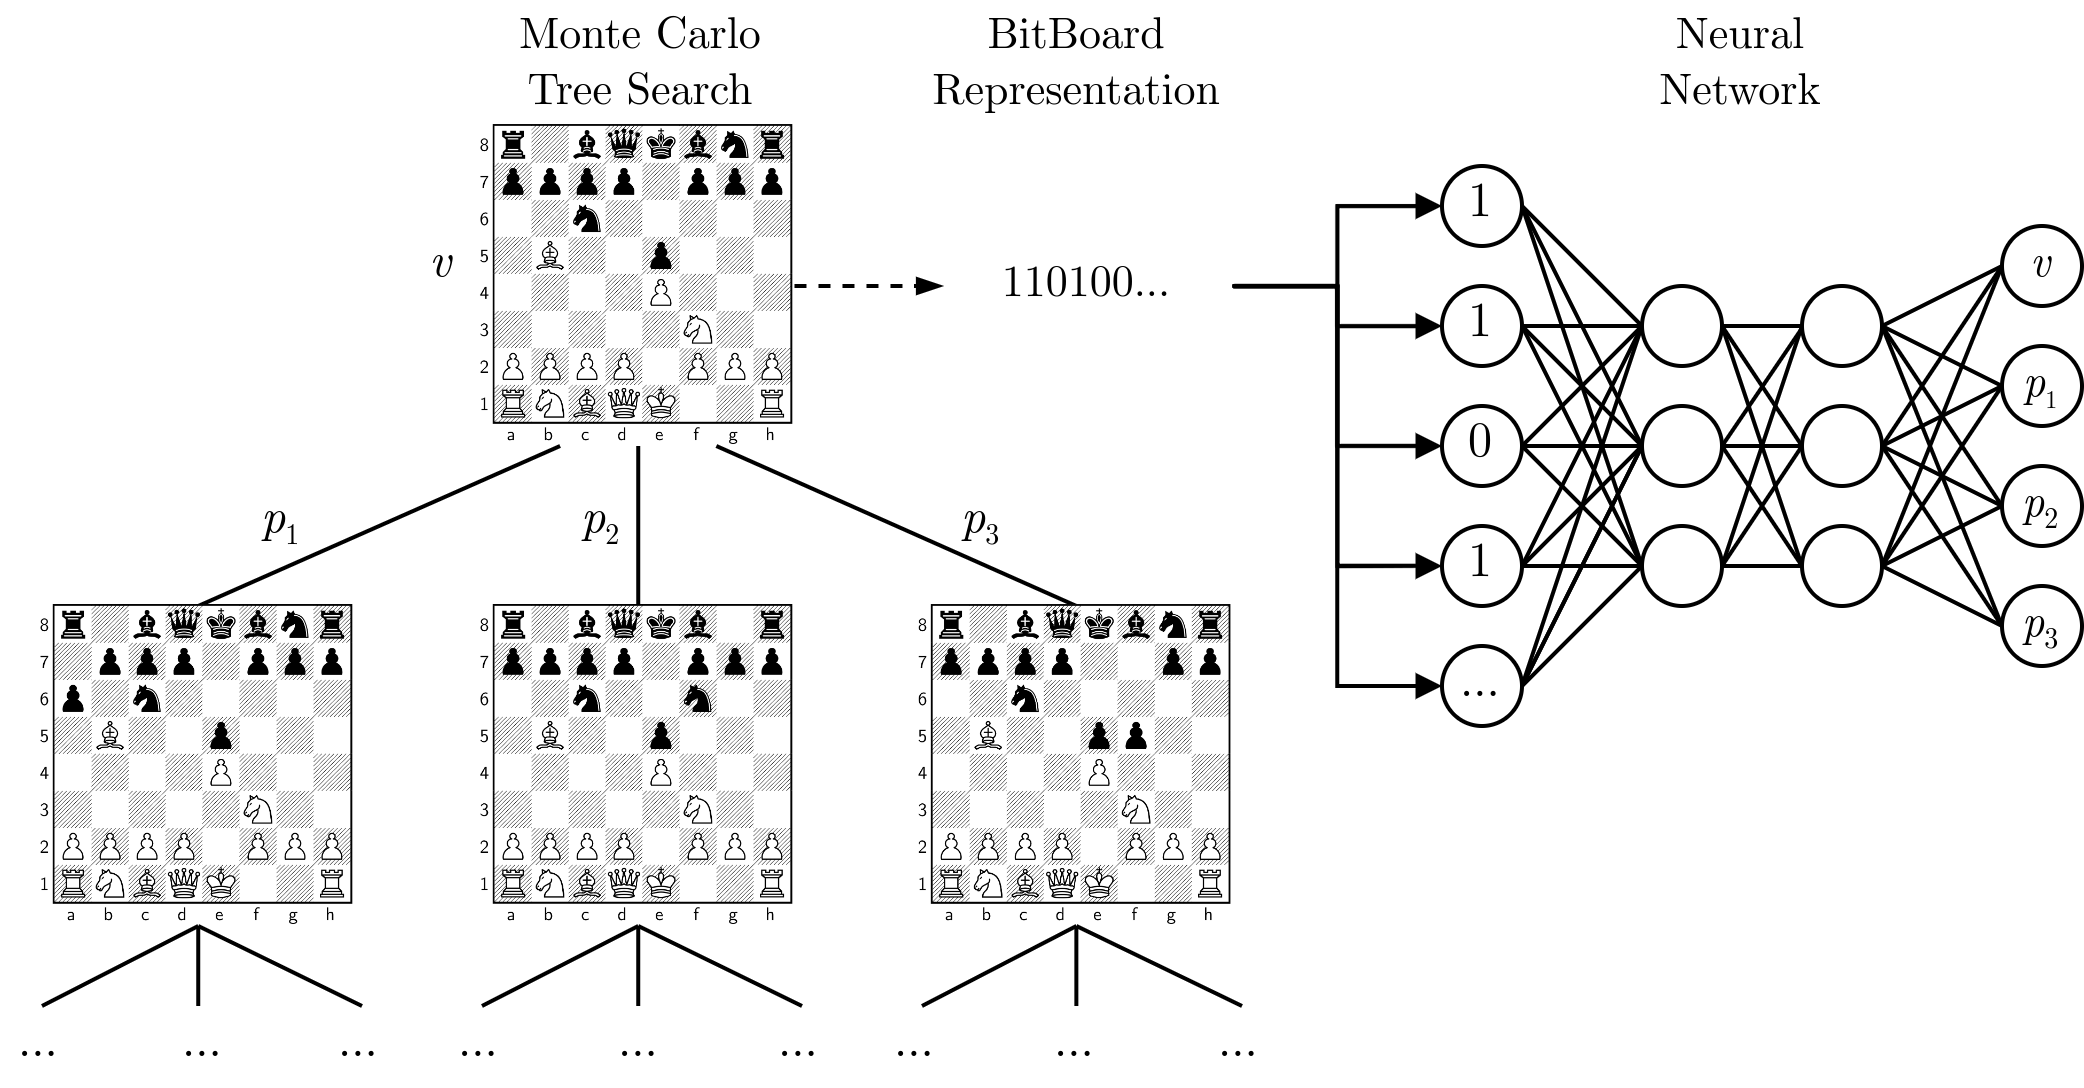
\includegraphics[width=0.95\textwidth]{graphics/alphazero/alphazero.png}
\caption{Simplified example of move search and position evaluation using MCTS and a neural network. ($p_{n}$ move probabilities, $v$ winning chance value)}
\end{figure}

In order for the neural network to deliver the best possible results, it must be trained with data. Instead of relying on existing data sets, \cite{alphazero-2018} used the approach of generating their own data sets through self-play. Initially a program exists that only knows the rules of the game, uses an untrained neural network for evaluation and the MCTS algorithm for move selection. The program executes the following four steps to train the neural network: (1) The program plays against itself by searching for several moves in advance through the MTCS, letting the neural network evaluate these moves for move probability and position strength, and finally choosing the path with the best evaluation. Every game is recorded move by move. At the end of each match, the final position of the sides are assigned lost (-1), drawn (0) or won (+1) to create a dataset.\footnote{See Silver et. al p. 2} (2) The neural network is cloned and the parameters are adjusted "to minimize the error between the predicted result [...] and the game result [...]" and train the network with the generated data set. (3) Let the new program play against the previous one. (4) The winning program is selected and the process is repeated from step 1. As \cite{alphazero-2018}  showed, this method was able to outperform Stockfish, the strongest engine at this time, after only 4 hours.

\begin{figure}[h]
\centering
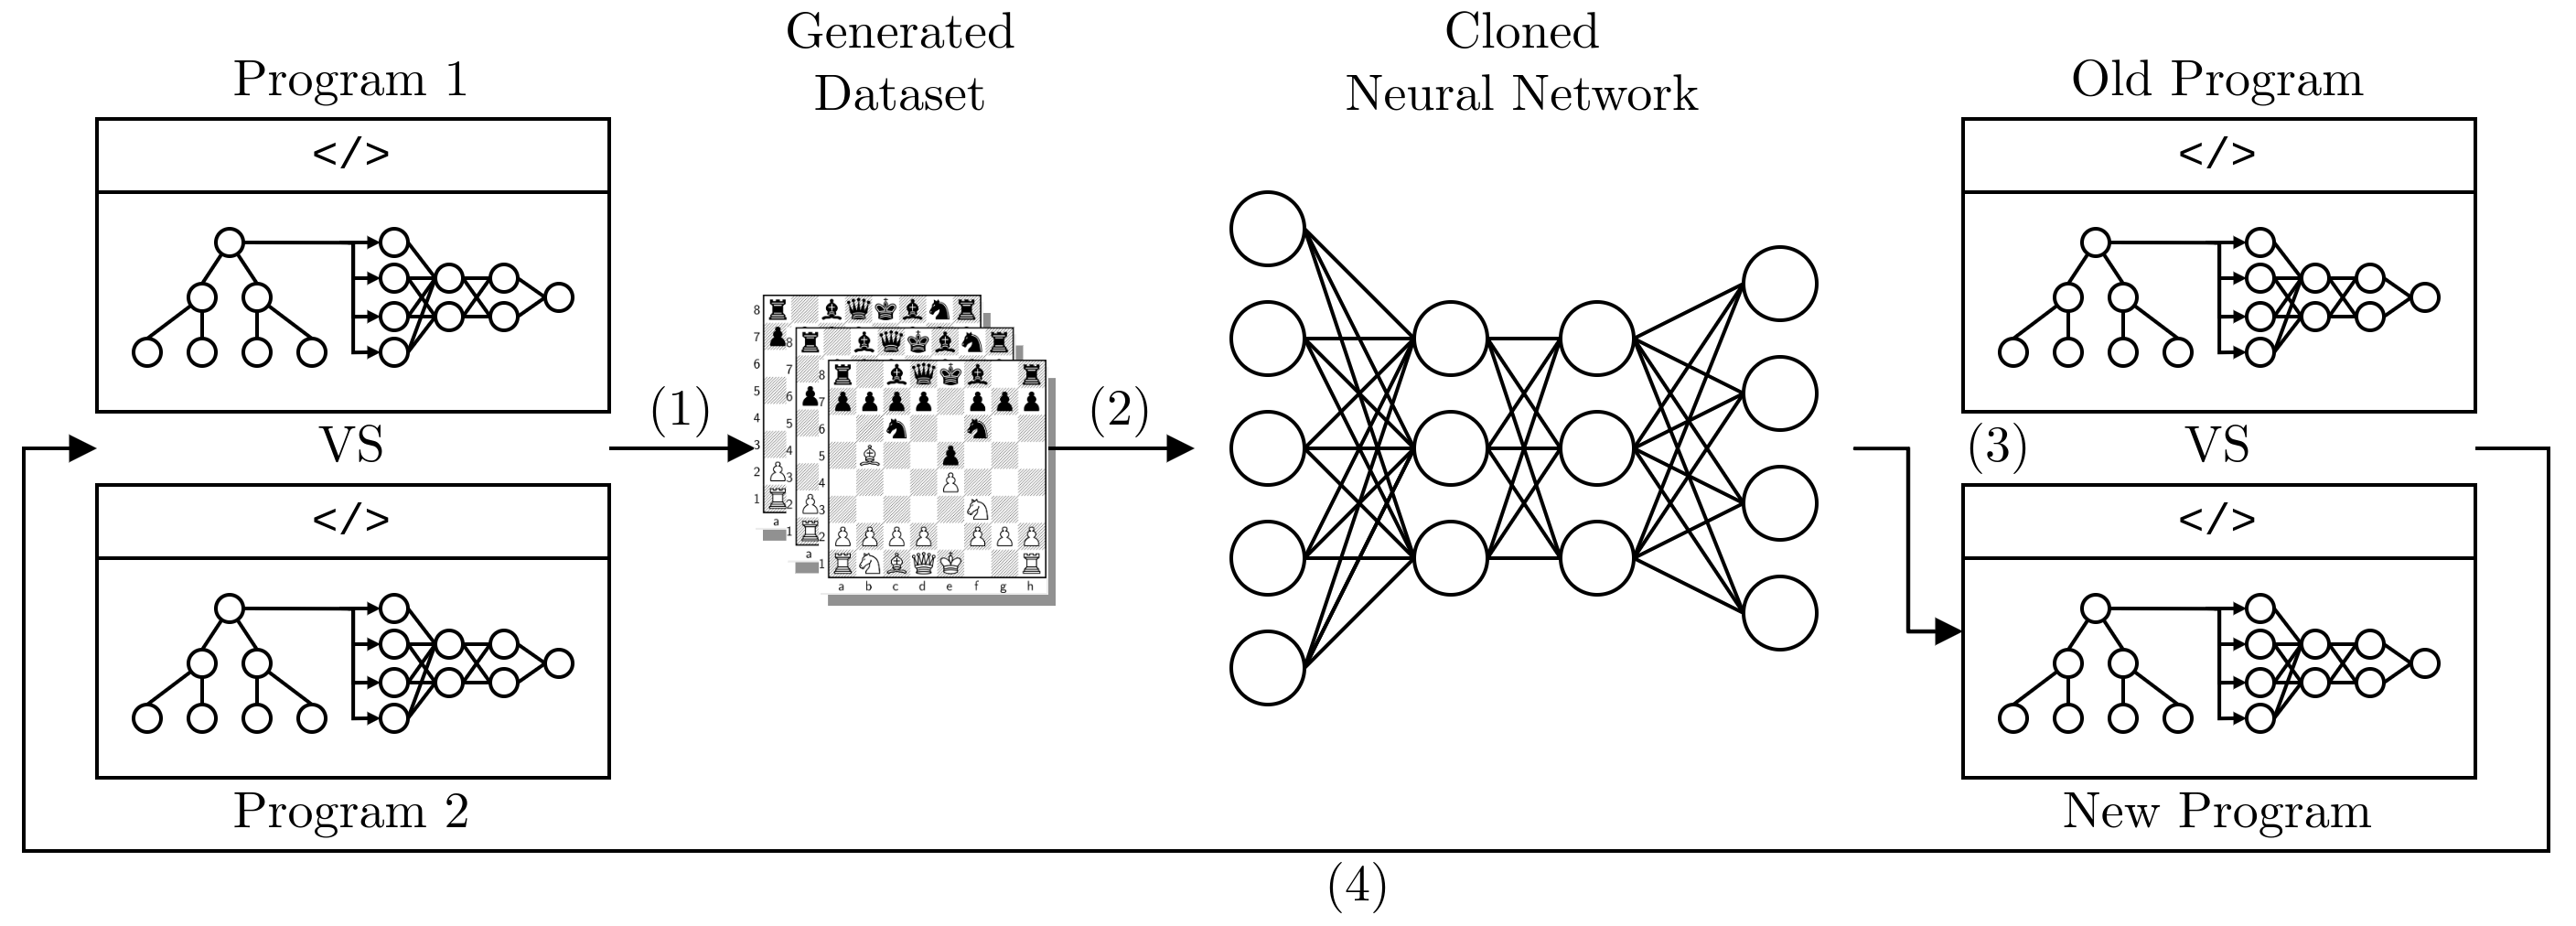
\includegraphics[width=0.95\textwidth]{graphics/alphazero/selfplay.png}
\caption{Steps of traning the neural network through self-play}
\end{figure}

% \subsubsection{State Evaluation}

% \subsection{Chess Commentator}

\newpage

\bibliographystyle{chicago}
\nocite{*}
\bibliography{references}

\end{document}

